\documentclass[../DoAn.tex]{subfiles}
\begin{document}
Chương 4 đã mô tả chi tiết hệ thống tích hợp dữ liệu, chương này sẽ trình bày kết quả đã làm, những đóng góp nổi bật cũng như tổng hợp những bài học kinh nghiệm trong suốt quá trình làm đồ án. Bên cạnh đó cũng trình bày hướng phát triển trong tương lai của hệ thống.

\section{Kết luận}
Hệ thống thu thập dữ liệu yêu cầu nguồn dữ liệu được bổ sung liên tục, các trang web bán hàng khác nhau được tích hợp lại để hỗ trợ đa dạng nhu cầu của người sử dụng. Do vậy, hệ thống này phải có tính mở rộng cao cho phép thêm các nguồn dữ liệu mới độc lập, dễ dàng triển khai. Để đáp ứng được yêu cầu cũng như hiện trạng trên em đã thiết kế xây dựng hệ thống độc lập hóa giữa các nguồn dữ liệu. Các nguồn dữ liệu khi được thêm mới vào hệ thống sẽ không có ràng buộc, ảnh hưởng đối với hệ thống đang chạy ổn định hàng ngày. Giải pháp được thực hiện để giải quyết vấn đề trên là xây dựng các lớp khác nhau, mỗi lớp ứng với một nguồn dữ liệu mới được thêm vào. Khi đó người lập trình sẽ tạo một class (lớp) với đầy đủ thông tin để thu thập dữ liệu bao gồm tên nguồn dữ liệu, đường dẫn gốc, cấu hình kafka để lưu trữ dữ liệu,... Người xây dựng hệ thống sẽ lập trình hàm thu thập dữ liệu chính từ trang web nguồn khai báo trước đó. Tương tự đối với các nguồn dữ liệu khác hoàn toàn độc lập so với hệ thống, có thể chạy song song đồng thời tăng hiệu suất của quá trình thu thập dữ liệu. Kết quả hê thống thu thập dữ liệu có 12 nguồn dữ liệu khác nhau được xây dựng thành 12 lớp thu thập dữ liệu hoàn toàn độc lập có thể chạy đồng thời song song cho thời gian xử lý cải thiện đáng kể so với chạy tuần tự.

\begin{figure}[H]
    \centering
    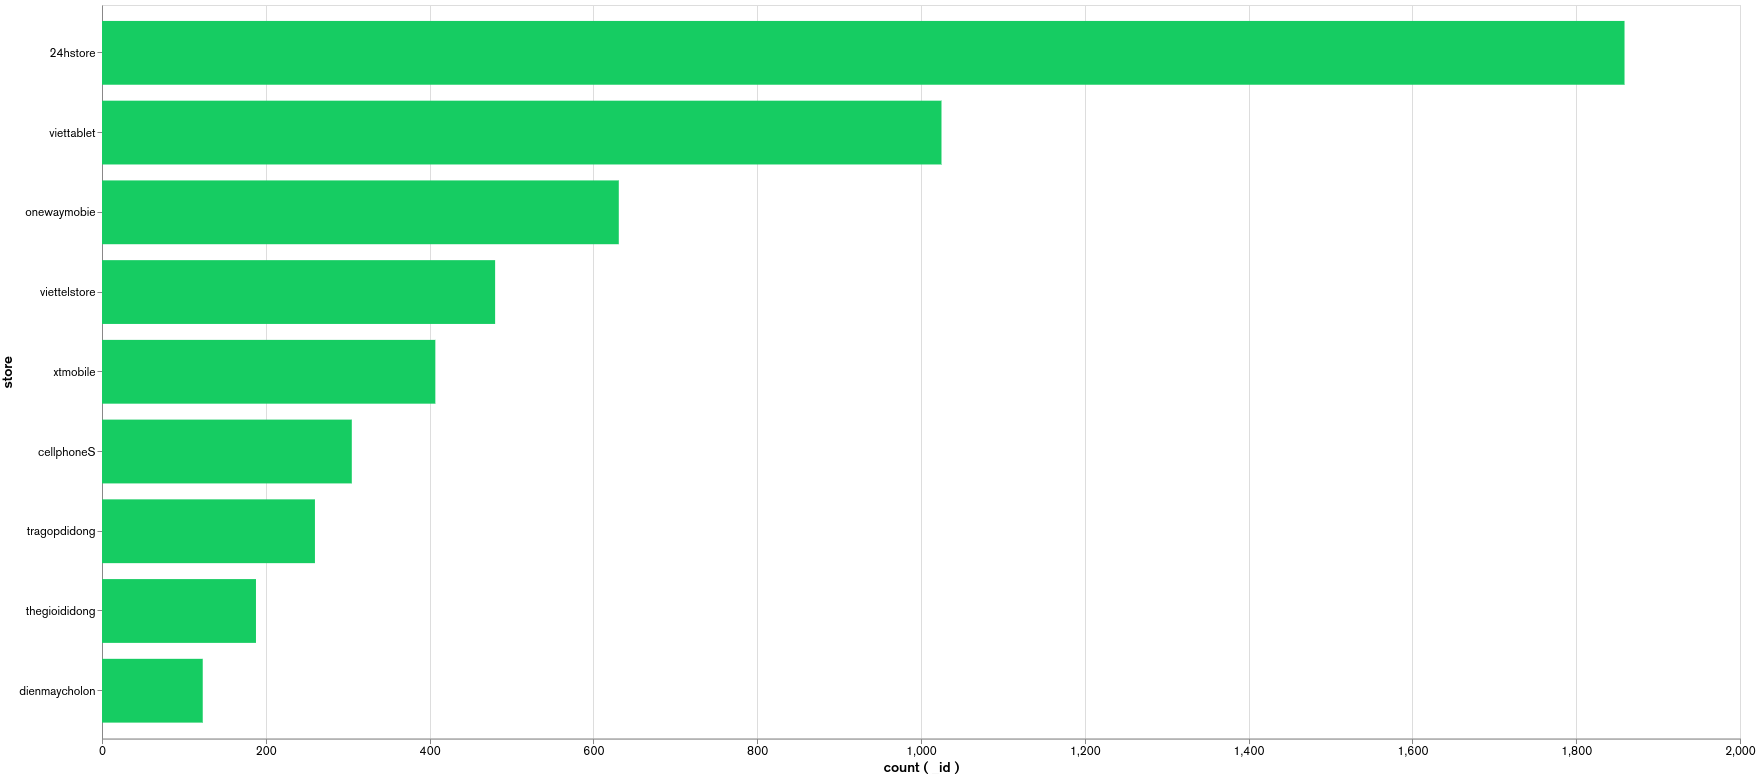
\includegraphics[scale=0.25]{Hinhve/total_items.png}
    \caption{Số lượng bản ghi sau khi xử lý}
    \label{fig:my_label2}
\end{figure}

Bên cạnh vấn đề mở rộng của hệ thống thì mức độ chịu lỗi cũng là một bài toán mà hệ thống tích hợp dữ liệu cần có để đảm bảo được luồng dữ liệu được tối ưu và tránh mất mát dữ liệu. Sau khi dữ liệu được thu thập hoàn toàn từ phía nguồn, hệ thống sẽ lưu trữ chúng tại các topic được định nghiã trong hệ thống Kafka và được lấy ra để xử lý ở những bước sau. Trong quá trình xử lý dữ liệu giả sử xảy ra lỗi ( có thể là lỗi môi trường, lỗi tích hợp dữ liệu sai định dạng, ...) thì thay vì chạy lại luồng từ pha thu thập dữ liệu hệ thống sẽ bỏ qua bước này và lấy dữ liệu trực tiếp từ kafka. Điều này giúp cho hệ thống được linh hoạt hơn chạy lại dữ liệu hàng ngày dễ dàng chỉ cần thao tác cấu hình mã nguồn, nơi đọc dữ liệu và tiến hành xử lý các bước sau. 

\begin{figure}[H]
    \centering
    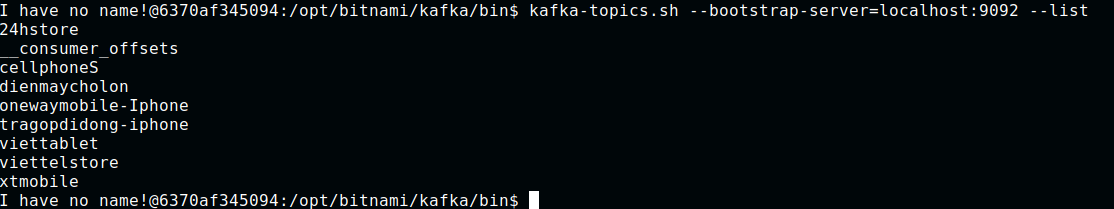
\includegraphics[scale=0.35]{Hinhve/kafka-topics.png}
    \caption{Các topics lưu trữ trong kafka}
    \label{fig:my_label2}
\end{figure}

Trong đồ án này, pha đóng vai trò quan trọng ảnh hưởng tới kết quả bài toán là pha tiền xử lý dữ liệu. Do vậy em tập trung và đưa ra những chiến lược tiền xử lý sao cho dữ liệu so khớp được đưa về định dạng chung thống nhất làm tiền đề cho pha so khớp dữ liệu ngay sau đó có độ chính xác cao. Phương pháp tiếp cận chủ yếu cho pha này như đã đề cập là ánh xạ từ một tập model đã được định nghĩa sẵn (được thu thập từ trang web). Bên cạnh đó do dữ liệu thu thập về dòng sản phẩm hẹp nên số lương thu thập được rất nhỏ và chứa nhiều trường giá trị rỗng, mặt khác qua quá trình khảo sát, phân tích nhận ra một điều là một số trường thông tin có chứa dữ liệu của trường khác cũng như chứa danh sách giá trị của nhiều sản phẩm nên chiến lược và phương pháp được đưa ra trích xuất thông tin từ những bản ghi này làm giàu cho dữ liệu. Kết quả tiền xử lý cho dữ liệu sạch và chuẩn định dạng đã thống nhất và đầy đủ trường thông tin.

Đóng góp chính của đồ án là xây dựng hệ thống tích hợp dữ liệu với khả năng linh hoạt mở rộng và tối ưu kiến trúc cũng như hiệu quả xử lý. Hệ thống này được thiết kế đàm bảo sao cho tối ưu các luồng xử lý không lặp lại và đưa ra được kết quả chính xác và kịp thời. Thật vậy với việc chia kiến trúc cơ sở dữ liệu thành 3 bảng khác nhau Product (sản phẩm), ProductSearch (Cụm sản phẩm), ProductDetail (Thông tin chi tiết của sản phẩm) trong đó bảng Product được cập nhật thường xuyên, 2 bảng dữ liệu còn lại là thay đổi chậm và chỉ được cập nhật sau một khoảng thời gian nhất định. Kiến trúc này giảm thời gian xử lý luồng dữ liệu đáng kể do nếu chạy cập nhật giá và phân cụm sau mỗi lần chạy thì hệ thống phải chạy thuật toán so khớp, nhóm cụm dữ liệu với độ phức tạp O(n*n). Thực tế hệ thống chạy hàng ngày chỉ cập nhật giá trong bảng Product, viêc cập nhât phân cụm sản phẩm còn tùy thuộc vào nhu cầu cũng như tốc độ thay đổi của thị trường có thể là 2-3 ngày hoặc 1 tuần.

\section{Hướng phát triển}

Hướng phát triển của hệ thống tích hợp dữ liệu hiện tại cần bổ sung thêm nhiều nguồn dữ liệu tin cậy từ khắp các trang bán hàng trực tuyến trên internet. Việc bổ sung này rất cần thiết phục vụ nhu cầu đa dạng của khách hàng cũng như giúp người dùng có nhiều góc nhìn lựa chọn phù hợp với họ. Hệ thống này đàm bảo bài toán mở rộng các nguồn dữ liệu là độc lập không ảnh hưởng tới ứng dụng đang chạy hàng ngày nên việc thêm nguồn dữ liệu là dễ dàng mở rộng và cập nhật. Bên cạnh đó bổ sung thêm chức năng ghi nhật kí các lần chạy luồng dữ liệu để theo dõi và giám sát hệ thống khi có lỗi kịp thời khắc phục, đảm bảo dữ liệu được chạy đúng, đủ. Đồng thời hệ thống cần tích hơp thêm nhiều loại dữ liêu khác nhau ví dụ như các dòng sản phẩm samsung, oppo,... hay mở rông hơn là các đồ dùng điện tử đang có mặt trên thị trường hay là việc bổ sung thêm những thông tin hữu ích khác như các bài đăng, bài bao liên quan đến sản phẩm giúp người dùng có thêm thông tin về sản phẩm từ đó đưa ra quyết định đúng đăn. Bài toán tích hợp dữ liệu mở rộng này không hề đơn gian đòi hỏi phải có quá trình khảo sát phân tích kĩ càng rồi mới đưa ra được phương pháp so khớp phù hợp. Ngoài ra, để phục vụ nhu cầu phân tích theo thời gian hệ thống cần có hạ tầng lưu trữ dữ liệu lịch sử của các sản phẩm.
Thay vì cập nhật lại giá sản phẩm hệ thống sẽ luu trữ dữ liệu theo partition của ngày, người dùng dùng có thể sử dụng thông tin này để phân tích dữ liệu lịch sử dự đoán xu hướng của thị trường.

Bên cạnh các công việc cần thiết để hoàn thiện các chức năng đã làm, hệ thống cần được phân tích các hướng đi mới cho phép cải tiến và nâng cấp hệ thống. Thật vậy, trong quá trình chạy luồng dữ liệu em có nhận thấy rằng do sử dụng selenium khá nhiều trong quá trình thu thập dữ liệu dẫn đến thời gian thu thập của hệ thống là khá lâu mặc dù đã chạy song song các nguồn dữ liệu khác nhau. Mặt khác scrapy là một framework mạnh trong việc thu thập và có tốc độ nhanh hơn nhiều so với scrapy. Vậy giải pháp ở đây đưa ra là thay thế selenium bằng scrapy ngay cả khi đó là một trang web động. Hệ thống sẽ tiến hành chạy bước thu thập url của các sản phẩm bằng selenium trước và lưu trữ vào cơ sở dữ liệu (coi như bảng này là thuộc loại ít thay đổi không chạy hàng ngày). Sau đó scrapy sẽ đọc địa chỉ url tại bảng đó và tiến hành thu thập bóc tách dữ liệu theo đúng như đã định nghĩa thực hiện luồng dữ liệu tuần tự. Cách tiếp cận này giúp cho hệ thống chạy nhanh hơn so với hệ thống cũ và ổn định. Ngoài việc tối ưu hệ thống thu thập dữ liệu cải thiện tốc độ, hệ thống cần có chiến lược tiền xử lý dữ liệu chặt chẽ hơn xử lý dữ liệu tổng quát đối với mọi đầu vào để làm sạch hướng tới pha so khớp dữ liệu cũng là một bước cần tối ưu. Có rất nhiều thuật tóan thư viện hỗ trợ bước so khớp dữ liệu này tuy nhiên mỗi một phương pháp có một ưu điểm nhươc điểm khác nhau do vậy có thể kết hợp các phương pháp này lại với nhau để tích hợp dữ liệu cho kết quả chính xác và nhanh chóng.



\end{document}